\chapter{Gestión de Procesos de Negocio}
%\section{FUNDAMENTO TEÓRICO} 
Se dedica este capítulo a presentar algunos conceptos que puedes ser básicos, pero que permiten la contextualización del problema de esta tesis.

%\section{Gestión de Procesos de Negocio}

\subsection{Proceso de negocio}

Aunque la definición de proceso es algo que está en la mente de cualquiera de los lectores, se define aquí un proceso de negocio como un conjunto de actividades ejecutadas en una secuencia específica, es decir, que tiene un flujo determinado por la lógica del negocio, los eventos externos y las reglas del negocio \citep{hitpass2017bpm}.

\subsection{Gestión de procesos de negocio}

BPM es el acrónimo de Business Process Management, en español: Gestión de Procesos de Negocio. Es una disciplina que integra un conjunto de principios, métodos y tecnologías con el propósito de contribuir al mejoramiento continuo del funcionamiento empresarial. La idea de BPM es hacer visible la gestión de los procesos de negocio y facilitar los cambios que sean requeridos \citep{smith2003business}. Según \citet{garimella2008introduccion}, BPM hace referencia a un conjunto de mejores prácticas de gestión de procesos, herramientas y tecnologías utilizadas para diseñar, representar, analizar y controlar los procesos del negocio, combinando las tecnologías de la información con metodologías de proceso y gobierno. BPM incluye el soporte integral de las tecnologías de información para mejorar, innovar y gestionar los procesos que determinan los resultados del negocio, crean valor para el cliente y facilitan el logro ágil de los objetivos del negocio” \citep{abpmp2013v3}.

\subsection{Suite de gestión de procesos de negocio bpms}

Un sistema o suite para la gestión de procesos de negocios (Business Process Management Suite (BPMS) “es un conjunto de herramientas de software que permiten modelar implementar y gestionar los procesos de negocio, que abarcan múltiples aplicaciones empresariales, departamentos y ``partners''”\citep{smith2003business}. Una Suite de Gestión de Procesos de Negocio está conformada por herramientas de software para la gestión de los procesos de negocios (diseño de procesos, flujo de trabajo, aplicaciones, integración y supervisión), los cuales son automatizados favoreciendo a las organizaciones \citep{underdahl2013gestion}.

\subsection{Modelo y notación de procesos de negocio}

Business Process Model and Notation (BPMN) es una herramienta gráfica estandarizada, para la notación del modelado de procesos de negocio, mediante un flujo de trabajo. La versión BPMN 2.0 fue presentada en el año 2011 \citep{omg2011business} y utiliza símbolos, relaciones y atributos para el modelado de procesos de negocio. Un ejemplo gráfico de cómo se ve un proceso modelado en BPMN se muestra en la figura \ref{EjBPMN}.

\subsection{Proceso de negocio dinámico y caso}

Es un proceso de negocio que no tiene un orden determinado para la ejecución de las actividades ni la certeza de cuáles de ellas se han de ejecutar, requiriendo la intervención de un experto \citep{hitpass2017bpmn}. A la tecnología que se encarga de la gestión de este tipo de procesos se le conoce momo gestión de “casos”; el caso contiene toda la información sobre el proceso \citep{marin2016introduction}.

\subsection{Notación para gestión de casos}

Case Management Model and Notation” – CMMN es una notación entregada por el grupo “Object Management Group” (OMG), como una notación gráfica para la gestión de casos y sus procesos dinámicos \citep{hauder2014research}; algunas de sus principales diferencias con la notación BPMN se ilustra en \citep{breitenmoser2015case}, y en \citep{marin2016introduction} se da una aplicación de esta notación a un sistemas de atención de quejas. \citet{auer2014business} ofrece un ejemplo del modelado de un proceso usando esta notación, el cual se aprecia en la figura \ref{EjCMMN}

\section{Conceptos básicos de Grafos}
Un grafo no es otra cosa que un conjunto de vértices (al menos uno) conectados entre ellos con aristas que pueden ser líneas o flechas. 

Es por esto que en su notación, básicamente se refieren dos conjuntos: el conjunto no vacío de los nodos o vértices N y el conjunto de las aristas A. Adicionalmente, puede ser necesario establecer una función entre las aristas y el producto cartesiano de los nodos, cuando el grafo no es sencillo, como se resume en la tabla \ref{tab:notgraf}.

\begin{table}[H] 
\caption{Notación para dos tipos de grafos}
\centering
\begin{tabular}{llll}
\textbf{TIPO}                        & \textbf{NOTACIÓN}                & \textbf{CARACTERÍSTICA}                    & \textbf{ARISTAS}                           \\ \hline
\multicolumn{1}{|l|}{Multigrafo}     & \multicolumn{1}{l|}{G = (N,A,f)} & \multicolumn{1}{l|}{Con aristas paralelas} & \multicolumn{1}{l|}{$f:A \rightarrow NxN$} \\ \hline
\multicolumn{1}{|l|}{Grafo sencillo} & \multicolumn{1}{l|}{G = (N,A)}   & \multicolumn{1}{l|}{Sin aristas paralelas} & \multicolumn{1}{l|}{$A \subseteq NxN$}               \\ \hline
\end{tabular}
\label{tab:notgraf}
\end{table}

Los grafos pueden ser dirigidos o no dirigidos, lo que gráficamente significa que sus aristas son flechas o líneas, respectivamente; si hay de ambas, se llaman grafos mixtos, como se aprecia en la tabla \ref{dirigido}.

\begin{table}[H]
\caption{Clasificación de grafos según sus aristas}
\centering
\begin{tabular}[c]{lcc}
\multicolumn{1}{c}{\textbf{TIPO}} & \textbf{DIBUJO}                      & \textbf{CARACTERÍSTICA}  \\ \hline
\multicolumn{1}{|l|}{Dirigido}    & \multicolumn{1}{l|}{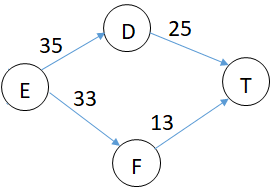
\includegraphics[align=t, width=36mm]{gafo dirigido.png} } &
%\multicolumn{1}{|l|}{Dirigido}    & \multicolumn{1}{l|}{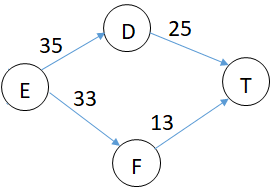
\includegraphics[width=27mm]{gafo dirigido.png} } &
\multicolumn{1}{p{6cm}|}{Todas sus aristas están dirigidas (flechas), que se pueden representar por parejas ordenadas (x,y)}     \\ \hline
\multicolumn{1}{|l|}{No dirigido} & \multicolumn{1}{l|}{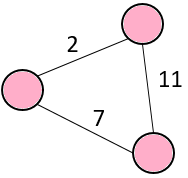
\includegraphics[align=t,width=36mm]{gafo no dirigido.png}} & \multicolumn{1}{p{6cm}|}{Todas sus aristas son no dirigidas (líneas), que se pueden representar por parejas no ordenadas \{x,y\}} \\ \hline
\multicolumn{1}{|l|}{Mixto}       & \multicolumn{1}{l|}{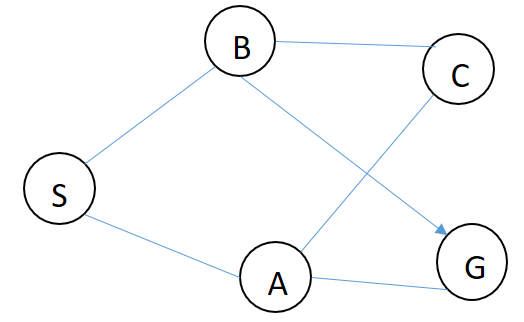
\includegraphics[align=t,width=36mm]{elementos de un grafo.png}} & \multicolumn{1}{p{6cm}|}{Contiene aristas dirigidas y aristas no dirigidas} \\ \hline
\end{tabular}
\label{dirigido}
\end{table}

Además, matemáticamente se hace una distinción en la representación de sus aristas, usándose parejas ordenas $(x,y) \in NxN$ para las aristas dirigidas y ${x,y} | (x,y) \in NxN$ para las aristas no dirigidas, lo que se puede interpretar como una doble flecha $(x,y)$ y $(y,x)$. Así que el contenido de la columna ARISTAS de la tabla \ref{tab:notgraf}, se refiere específicamente a aristas dirigidas \citep{tremblay1996matematica}.

También se habla de grafos completos, cuando contiene todas sus aristas posibles. Es decir, cada nodo tiene una arista para conectarse con cada uno de los demás existentes en el grafo. A medida que se aumenta el número de nodos en un grafo completa, su número de aristas aumenta en un progresión aritmética, porque se suma primero una, luego dos, luego tres, etc., siendo la cantidad que se suma inferior al número de nodos en una unidad, como se aprecia en la tabla \ref{cmpletos}

\begin{table}[H]
\centering
\caption{Los cinco primeros grafos completos}
\begin{tabular}[c]{|c|c|c|}
\hline
\textbf{Cantidad de nodos} & \textbf{Vista gráfica} & \textbf{Cantidad de aristas} \\ \hline
1 & \multicolumn{1}{l|}{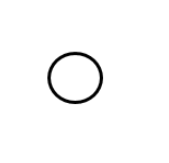
\includegraphics[align=t, width=27mm]{1nodo.png} }  & 0 \\ \hline
2 & \multicolumn{1}{l|}{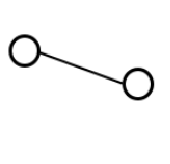
\includegraphics[align=t, width=27mm]{2nodos.png} }  & 1\\ \hline
3 & \multicolumn{1}{l|}{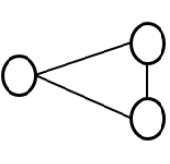
\includegraphics[align=t, width=27mm]{3nodos.png} }  & 3 \\ \hline
4 & \multicolumn{1}{l|}{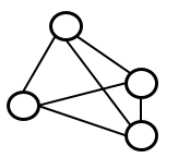
\includegraphics[align=t, width=27mm]{4nodos.png} }  & 6 \\ \hline
5 & \multicolumn{1}{l|}{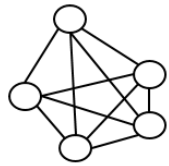
\includegraphics[align=t, width=27mm]{5nodos.png} }  & 10 \\ \hline
\end{tabular}
\label{cmpletos}
\end{table}

\section{Aprendizaje automático}
El Aprendizaje de Automático es una de las áreas de la Inteligencia Artificial que ha permitido extraer una importante cantidad de información, desde los datos que cada día se manejan en los negocios y en el mundo en general. Estos trabajos se han apoyado en diferentes técnicas como las redes Neuronales, los Algoritmos Genéticos, las Colonias de Hormigas, el Soporte de Máquina Vectorial y el Aprendizaje por Refuerzo, entre otras. En la tabla \ref{tipoML} se resume esta clasificación.

\begin{table}[H]
\caption{Tipos de aprendizaje automático}
\centering
\begin{tabular}{lc}
\multicolumn{1}{c}{\textbf{APRENDIZAJE}} & \textbf{CARACTERÍSTICA}                         \\ \hline
\multicolumn{1}{|l|}{Supervisado}        & \multicolumn{1}{c|}{Con datos de entrenamiento} \\ \hline
\multicolumn{1}{|l|}{No supervisado}     & \multicolumn{1}{c|}{Sin datos de entrenamiento} \\ \hline
\multicolumn{1}{|l|}{Por refuerzo}       & \multicolumn{1}{c|}{Premio o castigo}           \\ \hline
\end{tabular}
\label{tipoML}
\end{table}

El ML se encuentra catalogado en los textos como: aprendizaje supervisado, no supervisado o mixto, aunque el AR no se encuentra realmente en ninguna de estos tipos \citep{russell2004inteligencia}. 

En el aprendizaje supervisado el modelo aprende de acuerdo a unos datos de entrenamiento y posteriormente es capaz de reconocer patrones similares, mientras que, el aprendizaje no supervisado, no cuenta con datos de entrenamiento, sino que descubre automáticamente las características de los datos, logrando establecer, por ejemplo, las clases en las que pueden agruparse.

El AR se emplea en situaciones donde hay que tomar decisiones bajo incertidumbre, donde solo se conoce la consecuencia de una decisión, después de haberse tomado. Aquí se trata de entrenar un agente inteligente, el cual debe escoger la política que mejor resultado le dé, de acuerdo a las recompensas que recibirá de un ambiente donde se encuentra inmerso \citep{sutton1992reinforcement}.

\subsection{Los Bandits}
\label{Los Bandits}

El Multiarmed-Bandit es un modelo inspirado en las máquinas de un casino que se conocen con este nombre, donde se tienen cierto número de brazos, de los que se espera jugar los que mejor resultado alcancen y en el orden más adecuado. Cada máquina tiene su propia distribución de probabilidad, el jugador no las conoce inicialmente, pero a medida que va jugando, se va dando cuenta del resultado y va aprendiendo.

El modelo básico es el \textit{armed-bandit}, también conocido como \textit{bandit}, cuya analogía corresponde a una máquina de casino con un solo brazo o palanca, que en adelante se llamará acción. Para este modelo se tienen fórmulas sencillas que facilitan su implementación.

Por ejemplo, el beneficio acumulado que se recibe al seleccionar una acción “a” en diferentes tiempos i, es un promedio sencillo de las recompensas que el ambiente le reconoce al autómata al seleccionar dicha acción “a”, recompensa que no necesariamente será la misma en cualquier otra oportunidad o tiempo. La fórmula que se emplea es la fórmula \ref{Q}.
\begin{eqnarray}\label{Q}
Q_t(a) = \frac{R_1+R_2+ ...+R_{Nt(a)}}{N_t(a)}
\end{eqnarray}

Esta recompensa acumulada para cada acción, será afectada durante el aprendizaje del autómata y, la actividad que cuente con el mayor valor en su recompensa será la seleccionada o recomendada por el autómata o la aplicación.

El algoritmo de aprendizaje de los \textit{bandit}, es conocido como el algoritmo \textit{Q-learning}, el cual se explica en la figura \ref{AlgQ}.

\begin{figure}
  \centering
    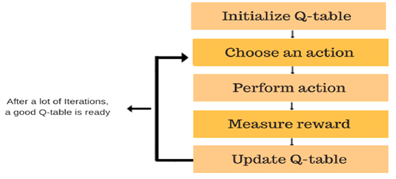
\includegraphics{Qlearning}
  \caption{Algoritmo \textit{Q-learning}. Fuente: \citep{ADL2018}}
  \label{AlgQ}
\end{figure}

Aquí \textit{Q-table}, se puede inicializar en cero para las recompensas de cada acción y se irá actualizando en forma recursiva, basándose en los valores futuros de la tabla, como se hace en programación dinámica, involucrando, por supuesto, la recompensa que el ambiente dará por la selección de la acción. De acuerdo al problema uno de estos dos valores tendrá mayor importancia: la recompensa futura o la actual, por lo que se cuenta con una variable que dará mayor peso a alguna de las dos, llamada $\gamma$, como se muestra en la fórmula \ref{Qsa}.
\begin{eqnarray}\label{Qsa} 
Q(s_t, a_t) = r(s_t, a_t) + \gamma max a_{t+1} Q(s_{t+1}, a_{t+1})
\end{eqnarray}

También implementa la estrategia $\epsilon$-greedy. El nombre de la estrategia obedece a que se cuenta con un parámetro $\epsilon$ con valores entre cero y uno, que le indicarán al agente si explota los valores de recompensa que está generando la acción que ha seleccionado o si mejor explota alguna de las otras acciones, de forma que evita que el agente se quede en la primera acción que le parezca buena, dando posibilidad a otras acciones. 

Al inicio el parámetro $\epsilon$ dará mayor importancia a la exploración, puesto que el agente no conoce todo el ambiente, y a medida que lo va conociendo le dará mayor peso a la exploración de la acción que ha selección porque ha encontrado mejores resultados, no sin dejar del todo la posibilidad de explorar otras acciones \cite{bubeck2012regret}.

%
%
De la revisión bibliográfica:

\begin{table}[H] 
\caption{Revisión de literatura - Grafos}
\centering
\begin{tabular}{cc}
\textbf{FUENTE}   & \textbf{DESCRIPCIÓN}   \\ \hline
\multicolumn{1}{|l|}{\citet{zhou2019toward}} & \multicolumn{1}{p{10cm}|}{Proponen mejoras a algoritmos de enrutamiento de ruta más corta (SPR), mediante sondeos de rutas múltiples y aprendizaje colaborativo.} \\ \hline
\multicolumn{1}{|l|}{\citet{liu2011multi}}   & \multicolumn{1}{p{10cm}|}{Recomendar la mejor ruta en un grafo, desde un origen hasta un destino donde el costo de cada enlace individual no se puede ver y el costo total de extremo a extremo solo se puede observar al finalizar el recorrido y está dado por la suma de los costos de todos los enlaces en la ruta. No hay etapas con nodos disyuntos.} \\ \hline
\multicolumn{1}{|l|}{\citet{liu2012adaptive}}   & \multicolumn{1}{p{10cm}|}{Aplican los principios del Bandido Multi-Brazos con brazos independientes al problema presentado por \citet{liu2011multi}} \\ \hline
\multicolumn{1}{|l|}{\citet{AvilaCartes2018}}   & \multicolumn{1}{p{10cm}|}{Problema \textit{Online Shortest Path Problem}, donde se usa un grafo dirigido y sin ciclos, con un nodo inicial y uno final o nodo sumidero. Haciendo uso de \textit{n-armed.bandit}, además de minimizar el costo con el camino que se seleccione, se desea disminuir la cantidad de veces que se escoge uno que presente fallas.} \\ \hline
\multicolumn{1}{|l|}{\citet{valko2016bandits}}   & \multicolumn{1}{p{10cm}|}{Recoge problemas de aplicación de grafos y \textit{bandits}, mostrando la aplicación de modelos que investigadores han desarrollado en problemas reales} \\ \hline
\multicolumn{1}{|l|}{\citet{tossou2017thompson}}   & \multicolumn{1}{p{10cm}|}{Algoritmo para problemas de decisión secuenciales, con grafos que presentan altos grados de incertidumbre, como alternativa para cuando las decisiones se tomaban basados en sencillos cálculos de probabilidades, quedando uno de dos eventos aceptado y el otro descartado.} \\ \hline
\end{tabular}
\label{tab:litera}
\end{table}

\begin{table}[H] 
\caption{Revisión de literatura - Aprendizaje por refuerzo}
\centering
\begin{tabular}{cc}
\textbf{FUENTE}   & \textbf{DESCRIPCIÓN}   \\ \hline
\multicolumn{1}{|l|}{\citet{lee2005reinforcement}} & \multicolumn{1}{p{10cm}|}{Propuesta para mejorar el tiempo de decisión de un algoritmo \textit{AQ-learnig} de aprendizaje por refuerzo con técnicas de inteligencia artificial de búsqueda por colonia de hormigas.} \\ \hline
\multicolumn{1}{|l|}{\citet{alon2017nonstochastic}}   & \multicolumn{1}{p{10cm}|}{Mediante los principios de Regresión, crean un espectro de modelos cuya complejidad está entre la de los problemas donde el agente conoce únicamente la recompensa de las acciones luego de elegirlas, y la de aquellos donde el agente tiene la información de lo que ocurrirá con cualquier acción candidata en cualquier instante.} \\ \hline
\multicolumn{1}{|l|}{\citet{alon2015online}}   & \multicolumn{1}{p{10cm}|}{Modelan el problema de un jugador aleatorio que se encuentra dentro de un ambiente que puede ser su adversario, quien después de cada acción recibe de sus vecinos información binaria del efecto de su acción.} \\ \hline
\multicolumn{1}{|l|}{\citet{gokcesu2018online}}   & \multicolumn{1}{p{10cm}|}{Presentan un algoritmo para \textit{n-armed bandits} con complejidad lineal que crece en función de la cantidad de secuencias posibles y del número de rondas del juego, sin el conocimiento del brazo que se debería escoger y sin suposiciones estadísticas.} \\ \hline
\multicolumn{1}{|l|}{\citet{8170860}}   & \multicolumn{1}{p{10cm}|}{Modelado de un problema de aprendizaje por refuerzo, mediante grafos, con un grafo en el que los nodos sí representan los brazos, pero las aristas tiene que ver con la similitud de sus valores de recompensas, aplicable a los sistemas de recomendación con baja complejidad} \\ \hline
\multicolumn{1}{|p{4cm}|}{\citet{silver2017mastering} y \citet{silver2016mastering}}   & \multicolumn{1}{p{10cm}|}{Aplicación de técnicas de aprendizaje por refuerzo para el entrenamiento de redes neuronales que lograron derrotar a los mejores jugadores humanos de ajedrez y Go, entre otros juegos, cada vez, con mejores resultados.} \\ \hline
\end{tabular}
\label{tab:litera}
\end{table}

